\subsubsection{Forwarding service}

This component is responsible of delivering messages from and to other nodes of
the system as a whole.

We show in figure \ref{fig:mw-forwarding} the architecture of this service and
then we will show in detail each module that composes this component.

\begin{figure}[H]
  \centering
  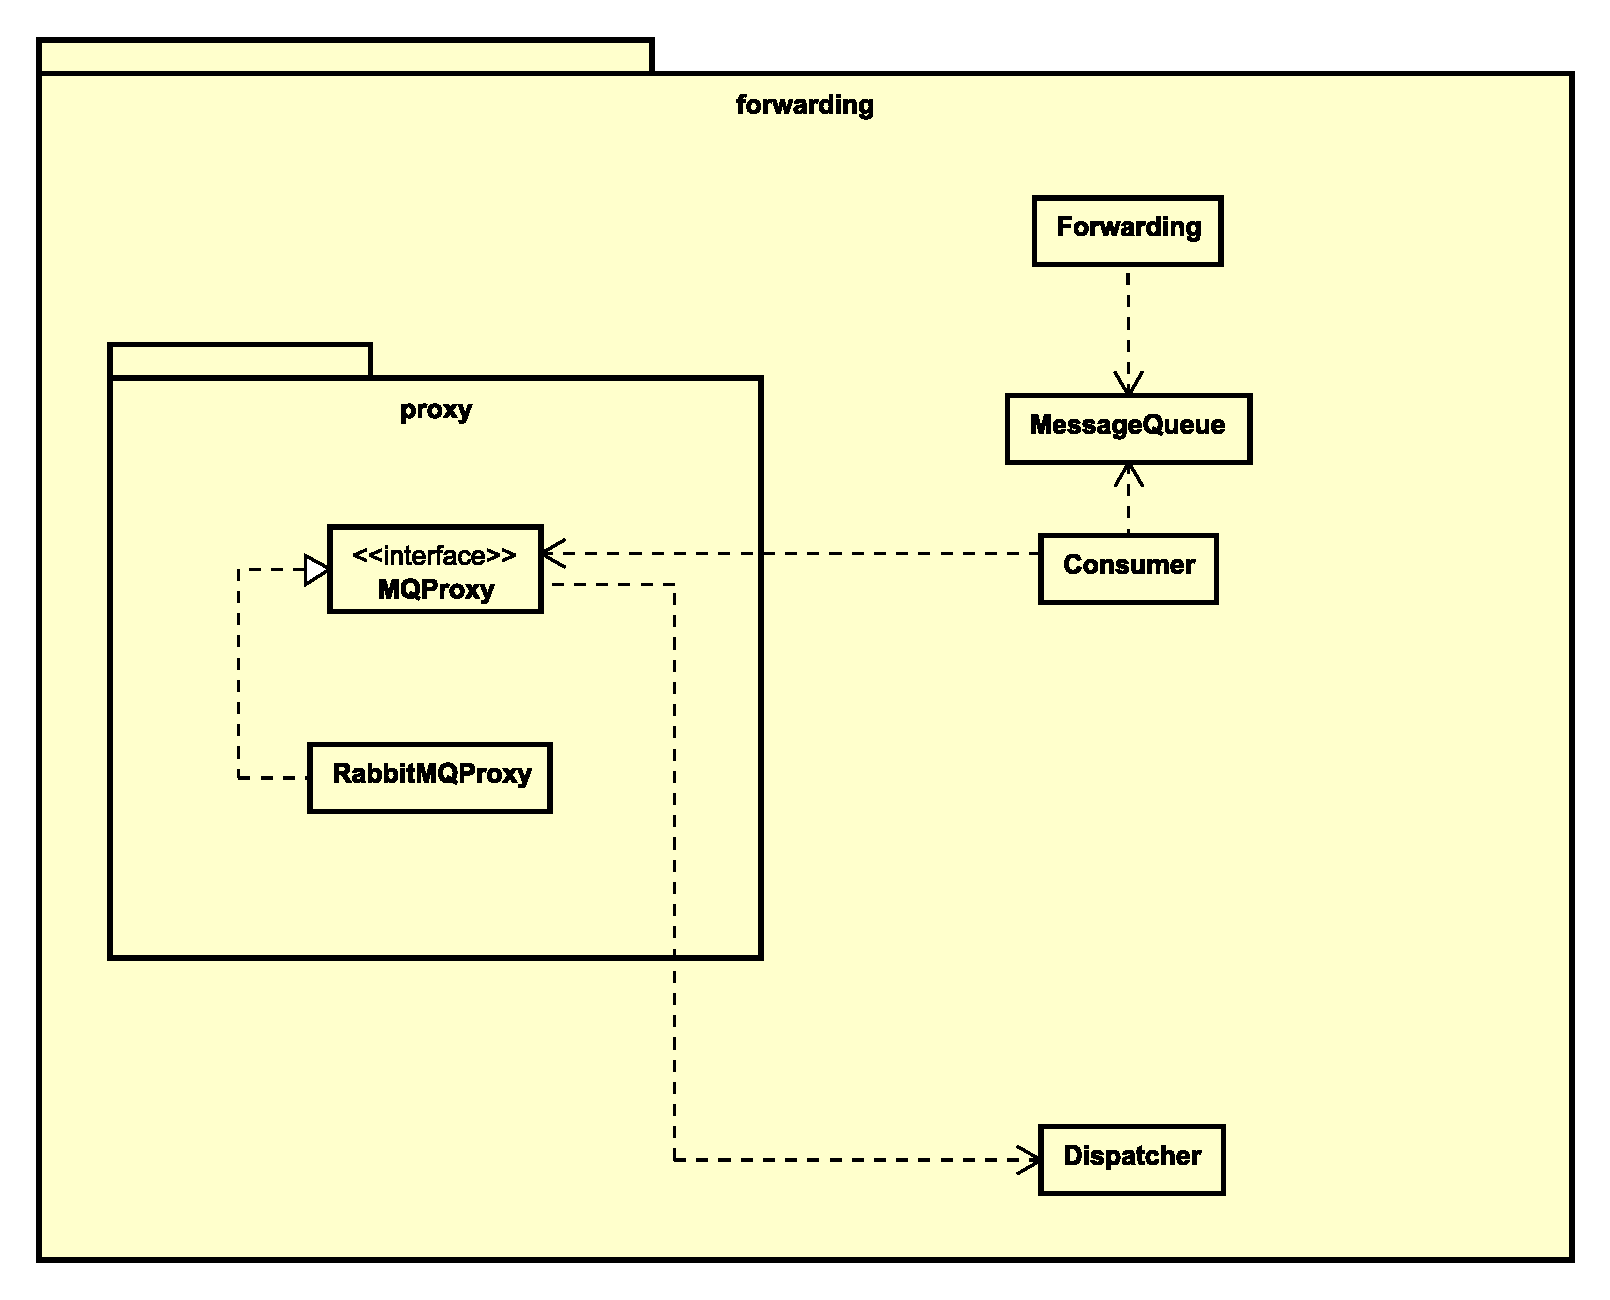
\includegraphics[width=\columnwidth]{images/solution/mw/forwarding.eps}
  \caption{Middleware's Forwarding service}
  \label{fig:mw-forwarding}
\end{figure}
% TODO: Can MessageQueue pass a message directly to Dispatcher if the message
%       is "local"?
% TODO: Change name of `Consumer to `MQConsumer

% TODO: All class diagrams have to be added
\subsubsubsection{forwarding.Forwarding}
% TODO: Class diagram
\FloatBarrier
\begin{itemize}
  \item \textbf{Description} \\
    This module is the Fa\c cade of the Forwarding service. It is responsible
    to boot neatly and supervise all processes in Forwarding. Also, it has to
    handle message delivery requests that come from other components of the
    middleware.
  \item \textbf{Attributes}
  \item \textbf{Operations}
  \begin{itemize}
    \item \texttt{+ start()} \\
    Starts the Forwarding service.
    \item \texttt{+ handleMessage(message: String)} \\
    % TODO: check this out: Message will really be a String?
    Handles the delivery of a given message to (possibly) other nodes.
  \end{itemize}
\end{itemize}

\subsubsubsection{forwarding.MessageQueue}
% TODO: Class diagram
\FloatBarrier
\begin{itemize}
  \item \textbf{Description} \\
    Process that has to pass messages to a forwarding.MQProxy.
  \item \textbf{Attributes}
    \begin{itemize}
      \item \texttt{- queue: AbstractQueue<Message>} \\
    Queue of messages.
      \item \texttt{- paused: Boolean} \\
    Value that is false iff the queue has to stop processing items due to
    some middleware operation (e.g. snapshot).
    \end{itemize}
  \item \textbf{Operations}
  \begin{itemize}
    \item \texttt{+ startLink(port: Int)} \\
    Starts the process and resume an eventual queue of messages from the
    last execution.
    \item \texttt{+ forward(message: String)} \\
    % TODO: check this out: Message will really be a String?
    Enqueue a message.
    \item \texttt{+ getHead()} \\
    Returns the first enqueued message, if present.
    \item \texttt{+ removeHead()} \\
    Removes the first enqueued message, if present.
    \item \texttt{+ pause(pausingMsg: String)} \\
    % TODO: check this out: Message will really be a String?
    Pauses the processing of enqueued messages. It also forwards this
    information to known nodes.
    \item \texttt{+ resume(resumptionMsg: String)} \\
    % TODO: check this out: Message will really be a String?
    Resumes the processing of enqueued messages. It also forwards this
    information to known nodes.
  \end{itemize}
\end{itemize}

\subsubsubsection{forwarding.MQConsumer}
% TODO: Class diagram
\FloatBarrier
\begin{itemize}
  \item \textbf{Description} \\
    Daemon worker that sequentially takes message from the MessageQueue to
    process them.
  \item \textbf{Attributes}
  \item \textbf{Operations}
  \begin{itemize}
    \item \texttt{+ waitToConsume()} \\
    Waits for new messages to be available in the MessageQueue.
  \end{itemize}
\end{itemize}

\subsubsubsection{forwarding.Dispatcher}
% TODO: Class diagram
\FloatBarrier
\begin{itemize}
  \item \textbf{Description} \\
    Dispatches incoming messages from the message broker.
  \item \textbf{Attributes}
  \item \textbf{Operations}
  \begin{itemize}
    \item \texttt{+ dispatch()} \\
    Dispatches the message to the intended middleware service.
  \end{itemize}
\end{itemize}

\subsubsubsection{forwarding.proxy.MQProxy}
% TODO: Class diagram
\FloatBarrier
\begin{itemize}
  \item \textbf{Description} \\
    Interface for processes that act in between middleware and a message
    broker.
  \item \textbf{Attributes}
  \item \textbf{Operations}
  \begin{itemize}
    \item \texttt{+ deliver(message: String)} \\
    % TODO: check this out: Message will really be a String?
    Makes the Message Broker deliver the message to the intended recipients.
  \end{itemize}
\end{itemize}

\subsubsubsection{forwarding.proxy.RabbitMQProxy}
% TODO: Class diagram
\FloatBarrier
\begin{itemize}
  \item \textbf{Description} \\
    Module that implements the \texttt{forwarding.proxy.MQProxy}
    interface to exchange messages with RabbitMQ.
  \item \textbf{Attributes}
  \item \textbf{Operations}
  \begin{itemize}
    \item \texttt{+ deliver(message: String)} \\
    % TODO: check this out: Message will really be a String?
    Delivers a message through the RabbitMQ message broker.
  \end{itemize}
\end{itemize}
